\documentclass{IOS-Book-Article}

\usepackage{times}
\normalfont
\usepackage[T1]{fontenc}
\usepackage[mtplusscr,mtbold]{mathtime}
\usepackage{epsfig}

\begin{document}
\begin{frontmatter}             

\title{Technology Neutral Business Process Design using URDAD}

\author{\fnms{Fritz} \snm{Solms}}
\address{Solms Training and Consulting CC, PostNet Suite 237, Private Bag X9, Melville, 2109, Johannesburg, South Africa; E-mail: fritz@solms.co.za.}
%\author[A]{\fnms{Fritz} \snm{Solms}}
%\address[A]{Solms Training and Consulting CC, PostNet Suite 237, Private Bag X9, Melville, 2109, Johannesburg, South Africa; E-mail: fritz@solms.co.za.}

\begin{abstract}
  This paper presents the Use Case, Responsibility Driven Analysis and Design methodology, URDAD.
  URDAD aims to provide a simple algorithmic design methodology which generates a technology neutral
  business process design in the context of model driven development. The design methodology has
  been formulated in such a way that it includes core drivers for widely accepted requirements for good design.
\end{abstract}

\begin{keyword}
URDAD, design methodology, model driven development, design principles, analysis, design,
technology neutral, MDA, business process design
\end{keyword}
\end{frontmatter}

\thispagestyle{empty}
\pagestyle{empty}


%=======================================================

\section{Introduction}

The aim of this paper is to present an implementable algorithmic analysis and design 
methodology which generates a technology neutral design model satisfying accepted
requirements for a ''good design''. The resultant model
is meant to represent the Platform Independent Model (PIM) of the
\textit{Model Driven Architecture} (MDA) published
by the Object Management Group (OMG), \cite{siegel:developingInMDA,frankel:enterpriseMDA}.

%--------------------------------------------------------------------

\subsection{Model driven development}

OMG's MDA forms the bases for most model driven development (MDD) 
processes\cite{selic:pragmaticsOfModelDrivenDevelopment,schmidt:modelDrivenEngineering}.
A high level view of a model driven approach
is shown in figure \ref{fig:modelDrivenApproach}.

\begin{figure}[hbt]
  \centering
  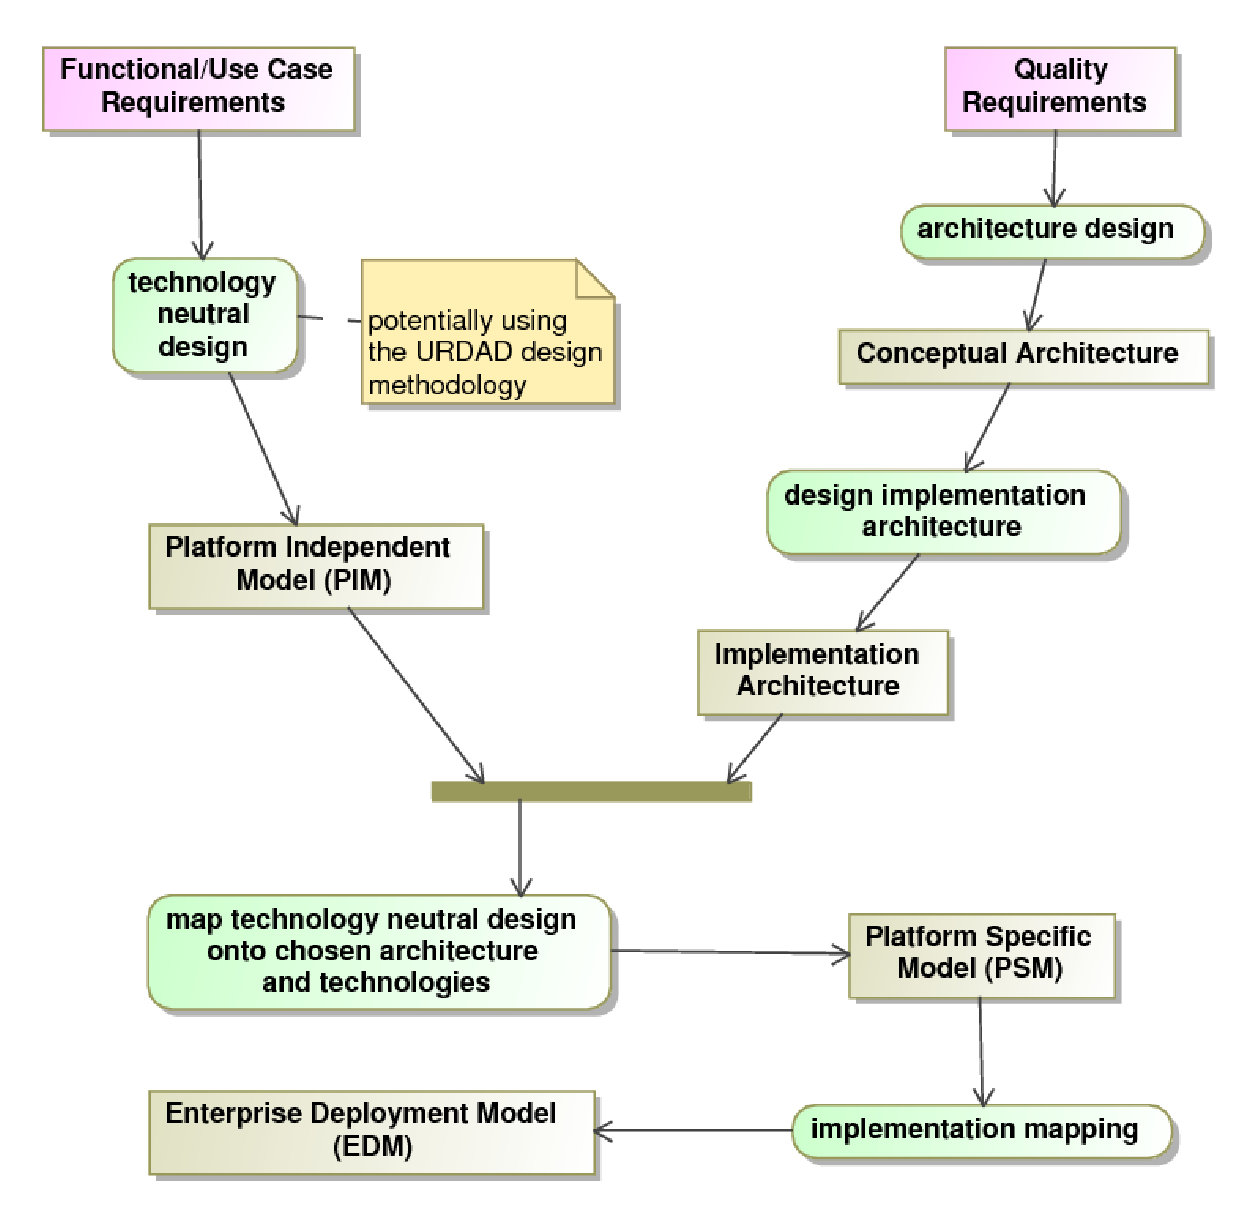
\epsfig{file=modelDriven.eps, scale=0.6}
  \caption{High level view of a model driven approach.}
  \label{fig:modelDrivenApproach}
\end{figure}

The input for the technology neutral business process design are the functional or use-case requirements. 
The output of the design phase is the Platform Independent Model (PIM) which can be mapped
onto one's choice of implementation architecture and technologies resulting in a Platform Specific
Model (PSM). Both, the PIM and the PSM are UML models. The Platform specific model is then taken
through an implementation mapping which includes the generation of all deployable artifacts including
the code, the database structures, the deployment scripts, the user documentation. MDA effectively
separates design from architecture.

URDAD targets
\begin{itemize}
  \item the analysis phase resulting in a use case contract, as well as  
  \item the design phase resulting in a technology neutral business process design.
\end{itemize}  
The use case contract contains both, functional and non-functional requirements around a use case. The
functional requirements drive the design process while the non-functional 
and in particular the quality requirements like scaleability, reliability, integrability, ... requirements 
drive the architectural process. The output of the architectural process is an 
infrastructure into which the business processes are to be deployed. 
This may span, both, organizational and systems architecture as business processes will often be realized 
across manual and automated processes
\footnote{The implementation mapping around manual business process steps would typically involve training of workers.}.

URDAD is usually embedded within an iterative realization or development process. 
A typical model driven development process is shown in figure \ref{fig:developmentProcess}. 
Note that the technology neutral business process design is performed by business analysis. 
The technical team comprising both, architecture and implementation (development), 
is responsible for the realization of the business process within the chosen architecture and technologies.

\begin{figure}
  \centering
  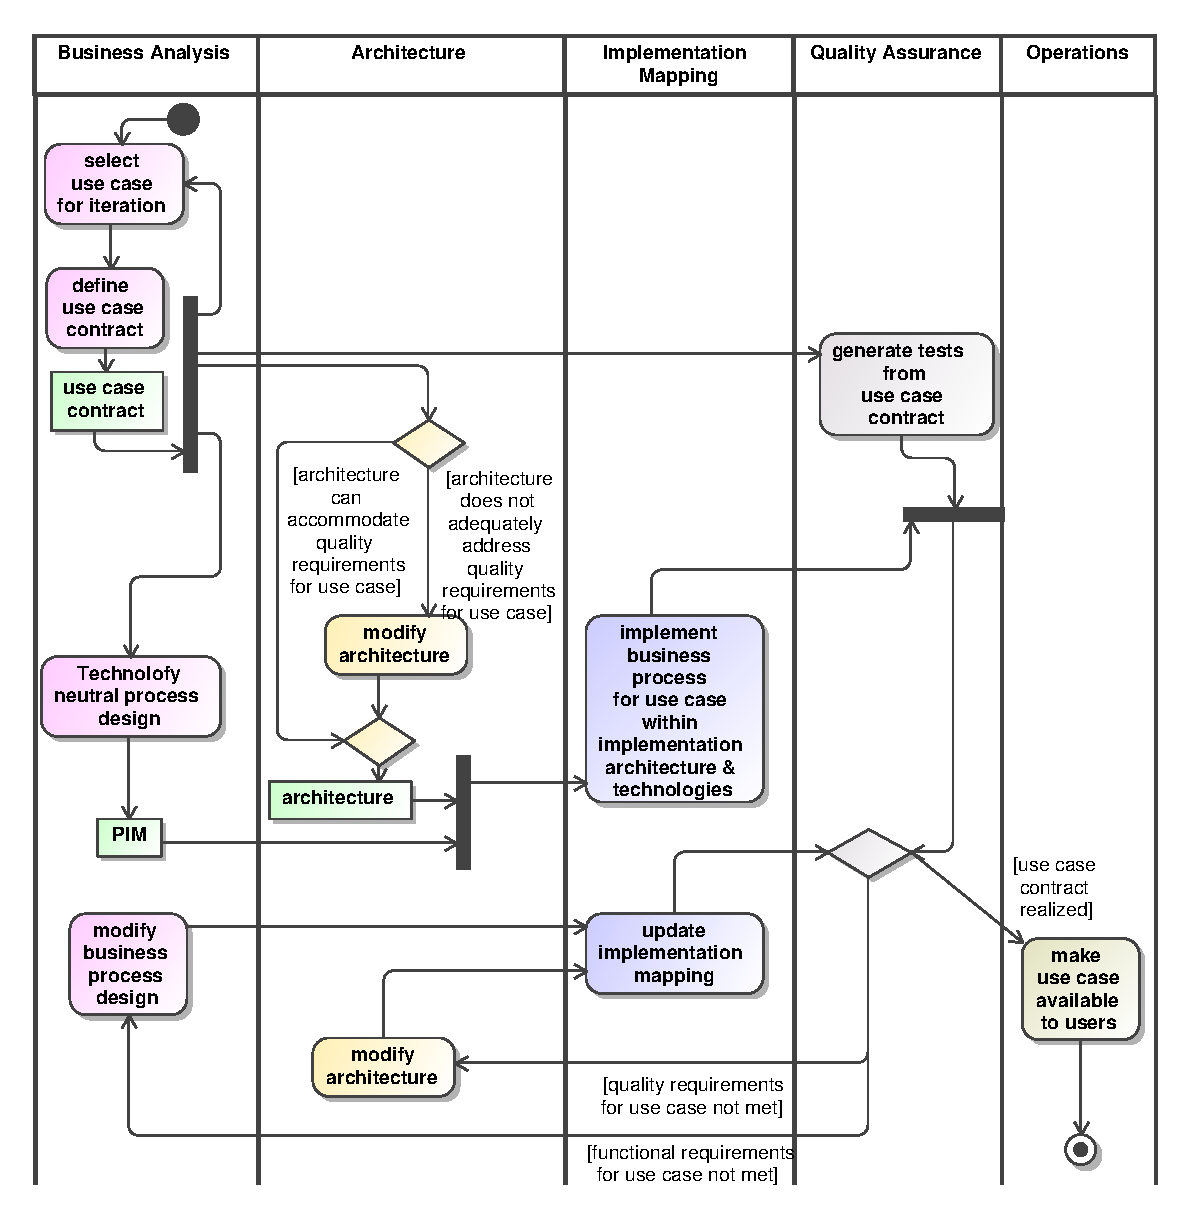
\epsfig{file=developmentProcess.eps, scale=0.6}
  \caption{Outline of a model driven development process.}
  \label{fig:developmentProcess}
\end{figure}

After passing quality assurance and actual deployment, operations takes over the management of the
business process execution.

%--------------------------------------------------------------------

\subsection{Requirements for the design methodology}

A good process design needs to fulfill the functional requirements of all the various stake
holders. The quality requirements (the non-functional requirements) are generally
addressed via architecture. For example, in order to achieve a specific level of scalability
and reliability one may decide on a clustered architecture supporting load balancing and
session replication. Any business process deployed in such an architecture would acquire
these qualities through the architecture -- these requirements need not be realized through 
process design.

Our aim was to formulate a design methodology which satisfies Berard's requirements for a methodology
\cite{berard:whatIsMethodology}. In particular, the methodology should represent an
engineering process which
\begin{itemize}
  \item can be used repeatedly, each time achieving similar results,
  \item can be taught to others within a reasonable time frame,
  \item can be applied by others with a reasonable level of success, 
  \item is applicable to a relatively large percentage of cases, and
  \item is able, on average, to achieve better results than either other techniques, or an ad hoc approach.
\end{itemize}

In order to generate ``good results'', one requires an understanding of the required attributes of a
``good design''. One can then attempt to identify design activities which ensure that the
design will have these desired attributes.

Robert C. Martin has compiled a widely quoted list of accepted design principles \cite{martin:agileSoftwareDevelopment}.
Many of these design principles including the interface segregation, dependency injection and the Liskov substitution
principles are realized by following a strict contracts based approach.
One of the most important principles is the single responsibility principle which requires that at any level of
granularity, each contract or class should address only a single responsibility. All the services should be narrowly aligned with the
this responsibility focus. The reuse/release equivalence principle can be addressed by enforcing that one only reuses
components which are released with realizing a published contract. If one would like to enforce the open-closed principle, one would do so
separately from a design methodology.

In addition to the design principles listed by Robert C.\ Martin, 
the generated design should also satisfy the simplicity principle, \cite{wirfs-brock:designSimplicity},
realize a high level of reusability \cite{lenz:softwareReuse},
exhibit clean layers of granularity, \cite{martin:agileSoftwareDevelopment, artus:soaRealization}
be testable across the levels of granularity \cite{voas:softwareTestability},
and facilitate bidirectional traceability across layers of granularity 
\cite{dick:designTraceability, aizenbud-reshef:modelTraceability}.

Figure \ref{fig:designActivities} shows  the final list of attributes we would want to 
realize within a design generated by the design methodology. 

\begin{figure}
  \centering
  \epsfig{file=designActivities.eps, scale=0.6}
  \caption{Design attributes and their dependencies on design activities.}
  \label{fig:designActivities}
\end{figure}


%=======================================================

\section{Other design methodologies}

URDAD has grown out of Responsibility Driven Design (RDD) methodology pioneered by Rebecca Wirfs-Brock and Brian Wilkerson (see \cite{wirfs-brock:responsibilityDrivenApproach},  and \cite{wirfs-brock:objectDesign} \cite{wirfs-brock:designSimplicity}). Like RDD, URDAD focuses during the early stages of the design on identifying and assigning responsibilities. Also, like RDD, URDAD puts a lot of emphasis on client-server contracts. URDAD adds a step-for-step algorithm which generates different layers of granularity, enforces decoupling within each level of granularity via work flow controllers and enforces, through the
methodology, a number of widely accepted design principles.

The {\em ICONIX} process from Doug Rosenberg discussed in \cite{rosenberg:useCaseDrivenObjectModeling} provide a structured process for evolving the static model from the collaboration requirements, but are not really responsibility driven, nor do they project out clean layers of granularity.

Methodologies like the Rational Unified Process \cite{kruchten:rup} and Extreme Programming are incorporate aspects of a design methodology, but are, in many respects
more software development than design methodologies.


%=======================================================

\section{Design activities realizing desired design attributes}

Figure \ref{fig:designActivities} also shows the design activities
which have been inserted into the design methodology in order to realize the
desired design attributes
as well as the dependency of design attributes on various design activities.
Each of these design activities has been directly built into the URDAD methodology:

%--------------------------------------------------------------------

\subsection{Enforce the single responsibility principle}

The single responsibility principle is enforced by grouping functional requirements into responsibility
domains and assigning each responsibility domain to a separate services contract. Any system or organizational
component as well as any external service provider realizing the full contract would be pluggable. Enforcing
the single responsibility principle directly drives pluggability and reusability. 

In addition, it makes each
object more understandable through being able to understand the contract(s) it realizes without having to 
understand the way in which the services specified in the contract are implemented.

Finally, enforcing the single responsibility principle also facilitates simpler maintainability as
\begin{itemize}
  \item maintenance is often required around a particular responsibility (enforcing the single responsibility
    principle leads to localized maintenance).
  \item One can verify whether, after maintenance work, the contractual obligations are still met.
\end{itemize}

%--------------------------------------------------------------------

\subsection{Fix the levels of granularity}

In the context of a work break down structure, one is automatically led to define different levels of granularity
\cite{demarco:structuredAnalysis}. In order to generate clean layers of granularity, URDAD starts by identifying the first
level responsibilities and assigns them to contracts. The business process
and ultimately the service provider contracts are specified for this level of granularity before going, 
in a structured way, to the next lower level of granularity.

This improves the maintainability of the design as changes to a business process often only need to be applied to the
controller of a particular level of granularity. 

Fixing the levels of granularity also improves the understandability and usability. It facilitates incremental understanding of 
a design, enabling one to look at a high level business process before specifying how each of the individual high level
work flow steps are realized through lower level business processes. Furthermore, a particular role player often only
needs to work at a specific level of granularity without there being a need to understand either the higher or lower levels
of granularity.

%--------------------------------------------------------------------

\subsection{Lock into contracts}

For each responsibility domain one assigns a separate services contract.
The business process is designed to be realized across abstract service providers realizing these contracts.
Design by contract rules are enforced ensuring the pluggability of service providers realizing the contract
as well as the pluggability of specializations. This results in a loosely coupled design.

Enforcing that service providers realize services contracts increases the reusability of such service providers
as the client can compare the services requirements with what is guaranteed through the contract.

Furthermore, enforcing contracts facilitates testability. It is difficult to write a sensible test if one does not know 
what the contractual obligations are which need to be tested.

A contracts based approach improves maintainability and extensibility through enhanced pluggability
and testability.

If all participants in a business process lock into contracts, the individual contracts can be realized within different
technologies. A contract driven approach can be used to generate a technology neutral design.

%--------------------------------------------------------------------

\subsection{Define for each level of granularity and each responsibility domain a controller}

Introducing for each level of granularity and each responsibility domain a controller localizes the business process
information within the controller and decouples the service providers from that level of granularity. Taking any 
business process decisions out of individual service providers and localizing it within a controller results in simpler 
business process management and maintenance\footnote{This strategy is also directly used within Services Oriented Architectures.}
Furthermore, the increased decoupling leads to a higher level of reusability. 

The introduction of a controller for each level of granularity also simplifies the design and improves understandability
as one only needs to look at the controller logic to understand the business process for the current level of granularity.

%--------------------------------------------------------------------

\subsection{Derive structure from process}

Going from a use case directly to defining structure is difficult and often leads to complexity which may not be required. 
A simpler approach which leeds to reduced complexity is that of defining first the process 
through which the use case is realized at a particular level of granularity. One can then project out
the minimal structure required to support the process.

Furthermore, driving structure from process facilitates the traceability of any structural element to the process it supports
and across the layers of granularity to the use cases for which it is required. Similarly, one can trace from a use case
to the structural elements required across the levels of granularity to realize the use case.

%--------------------------------------------------------------------

\subsection{Document relationships between layers of granularity}

Finally, documenting the relationships between the layers of granularity is required to support full
bidirectional traceability across the layers of granularity.

%=======================================================

\section{The URDAD methodology}

\begin{figure}[tb]
  \centering
  \epsfig{file=methodology.eps, scale=0.6}
  \caption{Outline of the URDAD methodology.}
  \label{fig:methodology}
\end{figure}

Having identified a use case or service one would like to realize, URDAD attempts to provide 
an algorithmic analysis and design methodology which incorporates the above design activities
in order to ensure that the resultant technology neutral business process design has the desired design attributes. The methodology starts with an initial analysis phase followed by a design phase
which incrementally generates a design across different levels of granularity.
The steps of the algorithm are shown in figure \ref{fig:methodology}.

This paper uses the example of processing an insurance claim to illustrate the algorithm. This example
is taken through two levels of granularity in order to illustrate the incremental refinement of the technology
neutral business process design.

%--------------------------------------------------------------------

\subsection{The analysis phase}

The analysis phase aims to elicit, verify and document the stake holder requirements. As one takes the business
process design through lower levels of granularity, one may require further input from the stake holders regarding
the detailed requirements around the lower level use cases.

%------------------------------

\subsubsection{Functional requirements}

During the analysis phase one first identifies all those stake holders who have an interest in the use case.
Each stake holder is prompted for their mandatory and conditional functional requirements around a use case.
Maintaining the linkage of any functional requirement to the stake holder who requires it facilitates full traceability
of any business or system activity back to the stake holder requirements they realize and ultimately to the 
stake holder itself.

\begin{figure}[thb]
  \centering
  \epsfig{file=processClaimUseCase.eps, scale=0.6}
  \caption{Functional requirements for the process claim use case.}
  \label{fig:processClaimUseCase}
\end{figure}

For example, figure \ref{fig:processClaimUseCase} shows the high level functional requirements for a process
claim use case. One can up-front elicit the requirements across levels of granularity or one can do that incrementally
in the context of designing the business process across layers of granularity. In the case where full 
functional requirements across levels of granularity are elicited up-front, the functional requirements would be
decomposed into lower level functional requirements. 

For example, the functional requirement of determining to what extend a policy covers a claim may include lower level
functional requirements like that of determining to what extend the contract covers the claim, assessing any
further constraints placed by public legislation and ultimately generating a claim coverage report. 

Often the detailed requirements around the different domains of responsibility are obtained from different role
players; i.e.\ while certain domains of business may be able to provide information around the higher level business
process, the details concerning lower level responsibilities are often determined from domain experts in the
appropriate domains of responsibility.
This can be done in the context of designing the lower levels of granularity of the business process.

%------------------------------

\subsubsection{User work flow}

The required user work flow is documented via interaction diagrams showing the messages exchanged 
between the subject responsible for realizing the use case and the actors. 

\begin{figure}[thb]
  \centering
  \epsfig{file=userWorkflowSuccess.eps, scale=0.6}
  \caption{The user work flow for a success scenario of the use case.}
  \label{fig:userWorkflowSuccess}
\end{figure}

For example, figure \ref{fig:userWorkflowSuccess}, shows the interactions of the subject with the actors for a particular
scenario and specifies the value objects exchanged between them.

%-------------------------------

\subsubsection{Business process requirements}

The business process as required by stake holders is specified using a high level activity diagram. 
It shows partitions for
the actors participating in the use case as well as a partition for the subject which is responsible for realizing the use
case. Note that this diagrams shows the required activities without specifying how they are realized within the subject.

\begin{figure}[thb]
  \centering
  \epsfig{file=userWorkflowGeneral.eps, scale=0.6}
  \caption{The general business process as required by the stake holders.}
  \label{fig:userWorkflowGeneral}
\end{figure}

Figure \ref{fig:userWorkflowGeneral} shows  example business process requirements for the process claim use case.

%--------------------------

\subsubsection{Exchanged value objects}

Part of the analysis phase is the specification of the exchanged value object.  For example, the policy holder receives
a settlement report. There will be a class diagram specifying the information which should be contained in the
settlement report.

In a similar way one specifies the information which must be provided with a claim, a payment request and a payment
confirmation. As we go through lower levels of granularity we may need to add further structure to some of the value
objects, particularly those which are provided by actors (e.g.\ the claim).

%--------------------------

\subsubsection{Adding pre- and post-conditions and quality requirements}

In order to be able to tale a full services contract view for the use case we need to assign pre- and post-conditions
as well as quality requirements to the use case. The pre-conditions are those conditions under which the service
may be refused without breaking the contract. 

The post-conditions are those conditions which must hold once the service has been provided. They apply to
the success scenarios of the use case.

Finally, there may be quality requirements which are specific to this use case. Quality requirements are non-functional
requirements referring to the realizable quality of service \cite{Bass:softwareArchitecture}. They refer to aspects like
scaleability, reliability, performance, integrability, ... and are the core drivers behind architecture and infrastructure.
While the pre- and post-conditions are part of the functional requirements which are realized through design,
the quality requirements are used to assess whether the target architecture for the use case
can indeed host the use case or whether architectural adjustments need to be made in order to realize the required
quality requirements.

\begin{figure}
  \centering
  \epsfig{file=processClaimPrePostQuality.eps, scale=0.6}
  \caption{Pre- and post conditions as well as quality requirements for the process claim use case.}
  \label{fig:processClaimPrePostQuality}
\end{figure}

Figure \ref{fig:processClaimPrePostQuality} shows an example of pre- and post-conditions as well as quality requirements
assigned to the ``buy product'' use case. 

%--------------------------------------------------------------------

\subsection{The design phase}

During an URDAD design phase one identifies the responsibilities for the current level of granularity,
assigns them to services contracts and specifies the business process the role players realizing the contract
need to execute. One then projects out the collaboration context, i.e.\ the static structure supporting the
collaboration which realizes the use case.

The output of the design phase is the technology neutral business process design for that level of granularity.

%--------------------------

\subsubsection{Responsibility identification and allocation}

During the first step of an URDAD design phase one groups functional requirements into  responsibility domains 
and assigns each responsibility domain to a separate services contract. 
Note that the technology neutral design specifies contracts for service providers
required within a business process.  
In the context of a model driven development process, the choice of a concrete
service provider or the technology within which a service provider is o be realized is made during the implementation 
mapping phase. A services contrac can be realized by a  system, an organizational component (e.g. a business 
unit) or an external service providers to whom the organization has outsourced 
certain responsibilities. 

\begin{figure}
  \centering
  \epsfig{file=processClaimResponsibilityAllocation.eps, scale=0.6}
  \caption{Responsibility identification and allocation for the process claim use case.}
  \label{fig:processClaimResponsibilityAllocation}
\end{figure}

URDAD requires that one adds the responsibility for managing the work flow and assigns the responsibility to
a separate services contract. This decouples the service providers from one another, localizes the business process
information for the current level of granularity and removes any business process information from the service
providers themselves. They are simply there to provide reusable services around a responsibility domain without
knowledge of the business processes for which these services are required.

Figure \ref{fig:processClaimResponsibilityAllocation} shows the responsibility identification and allocation for the
process claim use case.

%--------------------------

\subsubsection{Business process specification}

The services contracts are first introduced abstractly without specifying the services which service providers
realizing the services contract need to provide. Instead one next designs the business process for the current
level of granularity, showing how these abstract service providers need to collaborate in order to realize the use case.
The business process design feeds the services required for the business process into the services contracts for
the service providers required for the business process.

An interaction diagram like a sequence diagram is used to show how the role players from the current level of granularity
collaborate to realize the use case. It shows the messages value objects exchanged between these role players in a
technology neutral way. one can show multiple scenarios in a single diagram or use a separate sequence diagram
for any scenario which has significantly different interactions.

\begin{figure}[hbt]
  \centering
  \epsfig{file=processClaimSuccess.eps, scale=0.6}
  \caption{Role players collaborating to realize a success scenario of the process claim use case.}
  \label{fig:processClaimSuccess}
\end{figure}

Note that in figure \ref{fig:processClaimSuccess} the lowest level granularity messages are those between the controller and the service providers. Any
further messages exchanged in the context of these service providers realizing these service requests is deferred
to lower levels of granularity.

The full business process (see figure \ref{fig:processClaimBusinessProcess}) is then specified using an activity diagram with swim
lanes for each of the service providers participating in the current level of granularity.

\begin{figure}[htb]
  \centering
  \epsfig{file=processClaimBusinessProcess.eps, scale=0.6}
  \caption{The business process for the process claim use case (at the current level of granularity).}
  \label{fig:processClaimBusinessProcess}
\end{figure}
%--------------------------

\subsubsection{Projecting out the collaboration context}

The collaboration context shows the service providers required, at a specific level of granularity, to realize
the use case, the services they need to provide for this use case and the message paths we require in order
for the service providers to be able to collaborate to realize the use case.

Figure \ref{fig:processClaimCollaborationContext} shows the collaboration context for the process claim use case.
Note that the dynamics (i.e.\ the business process specification) will already have fed in the services required for
the business process into the contracts for the individual service providers. 

\begin{figure}[htb]
  \centering
  \epsfig{file=processClaimCollaborationContext.eps, scale=0.6}
  \caption{The collaboration context for the process claim use case.}
  \label{fig:processClaimCollaborationContext}
\end{figure}

%--------------------------------------------------------------------

\subsection{Transition to next level of granularity}

Having completed one analysis/design cycle, one needs to ask oneself whether
the business process for the use case has been fully specified or not. If not, one
may need to go to lower levels of granularity for some or all of the service
providers from the current level of granularity. \footnote{Often the lower level
granularity design is done by different business analysts who understand that domain
of responsibility (e.g.\ from a different department of the organization) or by the
business analysts of other organizations to whom the realization of the services 
contract is outsourced.}
This is done by selecting one of the service providers as the new context. The services
from the current level of granularity become the lower level use cases. After all, a use case
is defined as a service of value\cite{rumbaugh:umlReference}. One then selects a particular
service or use case and repeats the lower level analysis and design process.

Some of the information required we have already from the higher level granularity design phase.
This includes the user work flow, the stake holder requirements for the business process and
the specification of the value objects. However, one typically will need to do the 
identification of the lower level functional requirements and  specification of the 
formal contract parameters (the pre- and post-conditions and quality requirements).

Figure \ref{fig:assessCoverageFunctionalRequirements} shows an example of stake holders around
the lower level use case of assessing the policy coverage together with their functional requirements
around that use case.

\begin{figure}[htb]
  \centering
  \epsfig{file=assessCoverageFunctionalRequirements.eps, scale=0.6}
  \caption{Functional requirements for the assess coverage service.}
  \label{fig:assessCoverageFunctionalRequirements}
\end{figure}


The lower level design phase is executed in the same way as one was done for the higher level of granularity.
It start with the grouping of functional requirements into responsibility domains and the allocation of
each responsibility domain to a separate services contract. Figure \ref{fig:assessCoverageResponsibilityAllocation}
shows an example of identifying and allocating the lower level responsibilities around assessing the
policy coverage.

\begin{figure}[htb]
  \centering
  \epsfig{file=assessCoverageResponsibilityAllocation.eps, scale=0.6}
  \caption{Responsibility allocation for the assess coverage service.}
  \label{fig:assessCoverageResponsibilityAllocation}
\end{figure}

%--------------------------------

\subsubsection{Facilitating navigation across levels of granularity}

In URDAD a service from one level of granularity is mapped onto a use case at the next lower
level of granularity. In order to be able to conveniently navigate across levels of granularity,
one needs to maintain the link between the the service and its corresponding use case. This can
be done in various UML tools by adding a link with an appropriate stereotype.

%=======================================================

\section{How are the design activities realizing the desired design attributes embedded in URDAD?}

The single responsibility principle is directly enforced by grouping functional requirements into responsibility
domains and requiring the each responsibility domain is assigned to a separate contract.

The levels of granularity are fixed by including only those contracts to which the responsibilities for a
particular level of granularity have been assigned. Furthermore, the level of granularity is further fixed
be requiring that the lowest level service requests at a particular level of granularity are those which
come from the controller for that level of granularity.

The locking into services contracts is enforced by directly assigning responsibility domains to contracts and
specifying the work flow across these contracts. The URDAD design process then generates the 
contract details and requires the specification of pre-and post-conditions as well as quality requirements.

URDAD directly enforces the introduction of a work flow controller for each responsibility domain and
each level of granularity, resulting in the localization of the business process information and decoupling
of the service providers used in the business process.

The relationship between the layers of granularity are documented through an explicit transition across
the layers of granularity, facilitating bidirectional traceability.

Finally, the minimal conceptual (technology neutral) structure supporting the collaboration is projected out
from the dynamics of the business process realizing the use case.

%==========================================================

\section{Evaluating an URDAD based design}

In order to assess an URDAD based design one will
\begin{itemize}
   \item validate that each functional requirement is indeed adressed by the business process,
   \item assess the grouping of functional requirements into responsibility domains in
             order to verify that there are no overlaps between responsibility domains and that
             each responsibility domain does indeed comprise a single responsibility,
    \item  verify that the process at any level of granularity is intuitive and simple,
    \item verify that the service providers are represented by services contracts (UML interfaces) and 
              not by implementation or technology specific classes,
    \item verify that each services contract has been fully specified including the functional and
              non-functional requirements,
    \item verify that the structure of all exchanged value objects is defined using class diagrams.
\end{itemize}    

%=======================================================

\section{Implementation mappings}

The implementation mappings would be quite technology specific. Thus, while the technology neutral business process design
is usually done by business analysts, the implementation mappings are usually done by the technical team. 

Often a business process is realized across manual work flow steps, services provided by external service providers
and automated processing steps executed within systems. The services contracts coming out of the technology
neutral business process design can be used as a basis for the service provider contracts which are either realized
by external service providers or by business units hosted within the organization. The implementation mapping of
such work flow steps may require training certain staff members to execute them.

Often, however, the technology mapping may result in mapping the technology neutral design onto a realization using
current systems with perhaps some additional development, buying technology components and customizing them or 
developing an entire system hosting the various services. MDA tools aim to automate this process.

%----------------------------------------------------------------------------------

\subsection{Notes on mapping onto a service oriented architecture (SOA)}

In a services oriented architecture (SOA) \cite{erl:soa}
the work flow controllers for the various levels of granularity would map onto service specifications with 
higher level services being assembled from lower level services. The exchanged value objects would typically be
mapped onto  XML data structures usually specified using an XML schema. Some lower level services would be
realized not as composite services defined on a bus, but as atomic services which have been published on the
bus, but which are hosted in external systems.

%----------------------------------------------------------------------------------

\subsection{Notes on mapping onto a Java EE based architecture}

As a second example of a technology mapping, consider a typical Java EE architecture \cite{sun:javaee}.
The work flow controllers at the various levels of granularity would be typically mapped onto either session
or message driven beans. The value objects would map onto Java data objects or onto entity beans.

%=======================================================

\section{Conclusions}

The set of accepted design principles which are seen as required characteristics of a good design can
be supported by a set of design activities through which these design principles are realized. URDAD
defines an algorithmic design process which incorporates these design activities. It generates a
technology neutral business process design in the form of  services contracts for each level of granularity
together with the business process for that level of granularity. URDAD can be embedded within a
model driven development process where the technology neutral business process design is
ultimately mapped onto one's choice of implementation architecture and technologies.

%=======================================================

\section{Acknowledgments}

I would like to thank my college, Dawid Loubser, as well as
our clients and students. The many discussion we had
helped to solidify the vision and practical implementation of the
URDAD methodology.

%=======================================================

\bibliographystyle{abbrv}
\bibliography{urdad}  
\end{document}
